\documentclass[dvipdfmx,11pt]{beamer}

\usepackage[deluxe]{otf} 
\usepackage{txfonts}
\renewcommand{\kanjifamilydefault}{\gtdefault}
\usepackage{amssymb,amsmath}
\usepackage{hyperref}
\usepackage[absolute,overlay]{textpos}
\usepackage{comment}
\usepackage{colortbl}
\usepackage{graphicx}
\usepackage{tikz}
\usetikzlibrary{positioning}
\usetikzlibrary{shadows}
\usepackage{listings}
\usepackage{plistings}
\usepackage{multicol}
\def\lstlistingname{コード}
\newcommand{\code}[1]{\lstinline[basicstyle=\ttfamily]{#1}}
\newcommand{\lw}[1]{\smash{\lower-5.ex\hbox{#1}}}
\newcommand{\redunderline}[1]{\textcolor{red}{\underline{\textcolor{black}{#1}}}}

%%\usetheme{Frankfurt}
\usetheme{Warsaw}
\setbeamertemplate{navigation symbols}{} %スライドのボタン?(右下のやつ)を消す
\setbeamersize{text margin left=1.5em,text margin right=1.5em} % 余白なくすやつ

% footer setting %
\makeatother
\setbeamertemplate{footline}
{
  \leavevmode%
  \hbox{%
  \begin{beamercolorbox}[wd=.4\paperwidth,ht=2.25ex,dp=1ex,center]{author in head/foot}%
    \usebeamerfont{author in head/foot}\insertshortauthor
  \end{beamercolorbox}%
  \begin{beamercolorbox}[wd=.6\paperwidth,ht=2.25ex,dp=1ex,center]{title in head/foot}%
    \usebeamerfont{title in head/foot}\hspace*{1ex} \insertshorttitle\hspace*{3em}
    \textbf{ \insertframenumber{} / \inserttotalframenumber } \hspace*{1ex}
  \end{beamercolorbox}}%
  \vskip0pt%
}
\makeatletter

% exclude apprendix slides from framenumber %
\newcommand{\backupbegin}{
   \newcounter{framenumberappendix}
   \setcounter{framenumberappendix}{\value{framenumber}}
}
\newcommand{\backupend}{
   \addtocounter{framenumberappendix}{-\value{framenumber}}
   \addtocounter{framenumber}{\value{framenumberappendix}} 
}

\lstset{
 basicstyle=\ttfamily\color{black},
 keepspaces=true,
 escapechar=|,
 columns=[l]{fullflexible},
 commentstyle={\color{red}},
 stringstyle={\color{blue}}}

\title{解集合プログラミングを用いた\\配電網問題の解法}
\author[山田 健太郎,湊 真一,番原 睦則]{山田 健太郎$^1$,湊 真一$^2$,番原 睦則$^1$}
\date{\small 基盤(A)「離散構造処理系に基づく列挙と最適化の統合的技法の研究」\\
2020.09 プロジェクト近況報告&自由討論会}
\institute{1.名古屋大学 大学院情報学研究科 \\ 2.京都大学 大学院情報学研究科}

%#################################################
%# 本文 ##########################################
%#################################################
\begin{document}

%%%%%%%%%%%%%%%%%%%%%%%%%%%%%%%%%%%%%%%%%%%%%%%%%%
%% タイトル 
%%%%%%%%%%%%%%%%%%%%%%%%%%%%%%%%%%%%%%%%%%%%%%%%%%
\begin{frame}{}
  \titlepage
\end{frame}

%%%%%%%%%%%%%%%%%%%%%%%%%%%%%%%%%%%%%%%%%%%%%%%%%%
% 配電網
%%%%%%%%%%%%%%%%%%%%%%%%%%%%%%%%%%%%%%%%%%%%%%%%%%
\begin{frame}{配電網問題}
  \begin{alertblock}{}\centering
    求解困難な組合せ最適化問題の一種
  \end{alertblock}
  \vfill
  \begin{itemize}
  \item \alert{\bf 配電網}とは,変電所と,一般家庭や工場を繋ぐ電力供給
    経路のネットワークである.
  \item  配電網の構成技術はスマートグリッドや,災害時の障害箇所の迂回
    構成などを支える重要な基盤技術として期待されている.
  \item \alert{\bf 配電網問題}とは,
    \begin{itemize}
    \item \structure{\bf トポロジ制約}と\structure{\bf 電気制約}を満たしつつ,
    \item 損失電力を最小にするスイッチの開閉状態を求めることが目的.
    \end{itemize}
  \item これまで,メタヒューリスティクス等の解法が提案されている.
  \item 厳密解法としては,フロンティア法を用いた解法が提案されており
    \begin{itemize}
    \item 実用規模の配電網問題(\structure{\textbf{スイッチ数468個}})の
      最適解を求めることに成功~[井上ほか '12].
    \end{itemize}
  \end{itemize}
\end{frame}
%%%%%%%%%%%%%%%%%%%%%%%%%%%%%%%%%%%%%%%%%%%%%%%%%%
%% ASP
%%%%%%%%%%%%%%%%%%%%%%%%%%%%%%%%%%%%%%%%%%%%%%%%%%
\begin{frame}{解集合プログラミング(Answer Set Programming; ASP)}
  \begin{itemize}
  \item \structure{\bf ASPの言語}は一階論理に基づく知識表現言語の一種である.
  \item \structure{\bf ASPシステム}は論理プログラムから安定モデル意味
    論~[Gelfond and Lifschitz '88]に基づく解集合を計算するシステムである.
  \item 近年,SATソルバーの実装技術を応用した高速ASPシステムが実現され,
    システム検証,プランニング,システム生物学など様々な分野への応用が
    拡大している.
  \end{itemize}
  \vfill
  \begin{alertblock}{配電網問題に対してASP技術を用いる利点}
    \begin{itemize}
    \item ASP言語の高い表現力を生かし,各種制約を\textbf{簡潔に記述可能}
    \item マルチショットASP解法により,
      ある配電網構成(スタート状態)から他の配電網構成(ゴール状態)
      へのスイッチの切替手順を求める\textbf{遷移問題への拡張が容易}
    \item 背景理論つきASPにより,様々な\textbf{背景理論ソルバーと連携可能}
    \item 解の最適性を保証でき,最適解の列挙も可能
    \end{itemize}
  \end{alertblock}
\end{frame}
%%%%%%%%%%%%%%%%%%%%%%%%%%%%%%%%%%%%%%%%%%%%%%%%%% 
%% 根付き全域森問題
%%%%%%%%%%%%%%%%%%%%%%%%%%%%%%%%%%%%%%%%%%%%%%%%%%
\begin{frame}{根付き全域森問題}
  \begin{alertblock}{}
    トポロジ制約のみの配電網問題は,グラフと根と呼ばれる特別なノードから,
    \alert{\bf 根付き全域森}を求める部分グラフ探索問題に帰着できる.
  \end{alertblock}
  \vfill
  \begin{block}{根付き全域森 (Spanning Rooted Forest) [川原・湊 '12]}
    グラフ$G=(V,E)$と,
    \textbf{根}と呼ばれる$V$上のノードが与えられたとき,
    $G$上の根付き全域森とは,以下の条件を満たす$G$の部分グラフ$G'=(V,E'),\ E' \subseteq E$である.
    \begin{enumerate}
    \item $G'$はサイクルを持たない. (\alert{\bf 非閉路制約})
    \item $G'$の各連結成分は,ちょうど1つの根を含む. (\alert{\bf 根付き連結制約})
    \end{enumerate}
  \end{block}
\end{frame}
%%%%%%%%%%%%%%%%%%%%%%%%%%%%%%%%%%%%%%%%%%%%%%%%%%
%% 根付き全域森問題の例
%%%%%%%%%%%%%%%%%%%%%%%%%%%%%%%%%%%%%%%%%%%%%%%%%%
\begin{frame}{根付き全域森問題の例}
  \begin{columns}
    \begin{column}{0.45\textwidth}\centering
      \begin{exampleblock}{入力例}
	\centering
	%%%%%%%%%%%%%%%%%%%%%%%%%%%%%%%%%%%%%%%%%%%%%%%%%%
% 根付き全域森の例
%%%%%%%%%%%%%%%%%%%%%%%%%%%%%%%%%%%%%%%%%%%%%%%%%%

\begin{tikzpicture}[scale=0.5]

 % 設定
 \tikzset{node/.style={circle,draw=black,fill=white}}

 \definecolor{edge1}{RGB}{191,0,0}
 \definecolor{node1}{RGB}{249,200,200}
 \definecolor{edge3}{RGB}{38,38,134}
 \definecolor{node3}{RGB}{200,200,249}

 % 補助線
 % \draw [help lines,blue] (0,0) grid (20,6);

 % 入力されるグラフ
 % node %
 \node[circle, ultra thick,draw=edge1,fill=node1] (in1) {1};
 \node[node,right= of in1] (in2){2};
 \node[circle, ultra thick, draw=edge3,fill=node3, right=of in2](in3){3};
 \node[node,below= of in1] (in4){4};
 \node[node,below= of in2] (in5){5};
 \node[node,below= of in3] (in6){6};

 % 辺
 \foreach \u / \v in {in1/in2,in2/in3,in1/in4,in2/in5,in3/in6,in4/in5,in5/in6}
 \draw (\u) -- (\v);

\end{tikzpicture}

%%%%%%%%%%%%%%%%%%%%%%%%%%%%%%%%%%%%%%%%%%%%%%%%%%%%%%%%%%
%%% Local Variables:
%%% mode: japanese-latex
%%% TeX-master: ``slide''
%%% End:

      \end{exampleblock}
    \end{column}
    \begin{column}{0.05\textwidth}\centering
      $\Rightarrow$
    \end{column}
    \begin{column}{0.45\textwidth}\centering
      \begin{exampleblock}{解の例}
        \centering
        %%%%%%%%%%%%%%%%%%%%%%%%%%%%%%%%%%%%%%%%%%%%%%%%%%
% 根付き全域森の例
%%%%%%%%%%%%%%%%%%%%%%%%%%%%%%%%%%%%%%%%%%%%%%%%%%

\begin{tikzpicture}[scale=0.5]

 % 設定
 \tikzset{node/.style={circle,draw=black,fill=white}}

 \definecolor{edge1}{RGB}{191,0,0}
 \definecolor{node1}{RGB}{249,200,200}
 \definecolor{edge3}{RGB}{38,38,134}
 \definecolor{node3}{RGB}{200,200,249}

 % 補助線
 % \draw [help lines,blue] (0,0) grid (20,6);

 % node %
 \node[circle, ultra thick, draw=edge1, fill=node1](out1){1};
 \node[node, fill=node1, right=of out1] (out2){2};
 \node[circle, ultra thick, draw=edge3,fill=node3, right=of out2](out3){3};
 \node[node, fill=node1, below=of out1] (out4){4};
 \node[node, fill=node3, below=of out2] (out5){5};
 \node[node, fill=node3, below=of out3] (out6){6};

 \foreach \u / \v in {out1/out2,out1/out4}
 \draw [very thick, edge1] (\u) -- (\v);

 \foreach \u / \v in {out3/out6,out5/out6}
 \draw [very thick, edge3](\u) -- (\v);

\end{tikzpicture}

%%%%%%%%%%%%%%%%%%%%%%%%%%%%%%%%%%%%%%%%%%%%%%%%%%%%%%%%%%
%%% Local Variables:
%%% mode: japanese-latex
%%% TeX-master: ``slide''
%%% End:

      \end{exampleblock}
    \end{column}
  \end{columns}
  \vfill
  \begin{itemize}
  \item \structure{\bf 配電網とグラフの対応} \\
	 \begin{center}
      \begin{minipage}[c]{0.6\textwidth}
	   \begin{block}{}
		\centering
		\begin{tabular}{c|ccc}
		配電網 & 家庭 & スイッチ & 変電所 \\
		\hline
		グラフ & ノード & 辺 & 根
		\end{tabular}
	   \end{block}
      \end{minipage}
	 \end{center}\vfill
   \item \structure{\bf 配電網問題のトポロジ制約}
		 \begin{itemize}
		  \item 停電(変電所と結ばれない家庭)
		  \item 短絡(供給経路上のループ,複数の変電所と結ばれる家庭)
		 \end{itemize}
  \end{itemize}
\end{frame}
%%%%%%%%%%%%%%%%%%%%%%%%%%%%%%%%%%%%%%%%%%%%%%%%%%
%% 研究目的
%%%%%%%%%%%%%%%%%%%%%%%%%%%%%%%%%%%%%%%%%%%%%%%%%%
\begin{frame}{研究目的}
  \begin{alertblock}{目的}\centering
    ASP技術を活用して,大規模な配電網問題を効率良く解くシステムを構築
    する.
  \end{alertblock}
  \vfill
  \begin{block}{研究内容}
    \begin{enumerate}
    \item \structure{\bf 根付き全域森問題を解く2種類のASP符号化を考案}
      \begin{itemize}
      \item 基本符号化
      \item 改良符号化
      \end{itemize}
    \item 根付き全域森問題のある解(スタート状態)から他の解(ゴール状態)
      への辺の切替手順を求める\structure{\bf 解の遷移問題への拡張}
      \begin{itemize}
      \item シングルショット符号化
      \item マルチショット符号化
      \end{itemize}
    \item \structure{\bf 実用規模の問題,および,より大規模な問題を用いて評価}
    \end{enumerate}
  \end{block}
\end{frame}
%%%%%%%%%%%%%%%%%%%%%%%%%%%%%%%%%%%%%%%%%%%%%%%%%%
%% 提案手法
%%%%%%%%%%%%%%%%%%%%%%%%%%%%%%%%%%%%%%%%%%%%%%%%%%
\begin{frame}{提案手法}
   \scalebox{0.9}{\centering  \thicklines
  \setlength{\unitlength}{1.28pt}
  \small
  \begin{picture}(280,57)(4,-10)
    \put(  0, 20){\dashbox(50,24){\shortstack{根付き全域森\\問題}}}
    \put( 60, 20){\framebox(50,24){変換器}}
    \put(120, 20){\dashbox(50,24){\shortstack{ASPファクト}}}
    \put(120,-10){\alert{\bf\dashbox(50,24){\scriptsize{\shortstack{ASP符号化\\(論理プログラム)}}}}}
    \put(180, 20){\framebox(50,24){ASPシステム}}
    \put(240, 20){\dashbox(50,24){\shortstack{根付き全域森\\問題の解}}}
    \put( 50, 32){\vector(1,0){10}}
    \put(110, 32){\vector(1,0){10}}
    \put(170, 32){\vector(1,0){10}}
    \put(230, 32){\vector(1,0){10}}
    \put(170, +2){\line(1,0){4}}
    \put(174, +2){\line(0,1){30}}
  \end{picture}  
}
   \begin{block}{2種類のASP符号化を考案}
     \begin{itemize}
     \item \alert{\bf 基本符号化}
       \begin{itemize}
       \item 根付き全域森問題の制約を,\textbf{ASPのルール7個}で簡潔に記述
       \end{itemize}
     \item \alert{\bf 改良符号化}
       \begin{itemize}
       \item ASPシステムは,変数を含む論理プログラムを,変数を含まない
         論理プログラムに\textbf{基礎化}したのち解集合を計算する.
       \item 根付き連結制約をASPの個数制約で表現することにより,
         \textbf{基礎化後のルール数を少なく抑える}よう工夫されている.
       \item これにより,改良符号化は大規模な問題への有効性が期待できる.
       \end{itemize}
     \end{itemize}
   \end{block}
\end{frame}
%%%%%%%%%%%%%%%%%%%%%%%%%%%%%%%%%%%%%%%%%%%%%%%%%%
%% ASPファクト表現
%%%%%%%%%%%%%%%%%%%%%%%%%%%%%%%%%%%%%%%%%%%%%%%%%%
\begin{frame}{根付き全域森問題のASPファクト表現}
 \begin{figure}
  \centering
  %%%%%%%%%%%%%%%%%%%%%%%%%%%%%%%%%%%%%%%%%%%%%%%%%%
% 根付き全域森の例
%%%%%%%%%%%%%%%%%%%%%%%%%%%%%%%%%%%%%%%%%%%%%%%%%%

\begin{tikzpicture}[scale=0.5]

 % 設定
 \tikzset{node/.style={circle,draw=black,fill=white}}

 \definecolor{edge1}{RGB}{191,0,0}
 \definecolor{node1}{RGB}{249,200,200}
 \definecolor{edge3}{RGB}{38,38,134}
 \definecolor{node3}{RGB}{200,200,249}

 % 補助線
 % \draw [help lines,blue] (0,0) grid (20,6);

 % 入力されるグラフ
 % node %
 \node[circle, ultra thick,draw=edge1,fill=node1] (in1) {1};
 \node[node,right= of in1] (in2){2};
 \node[circle, ultra thick, draw=edge3,fill=node3, right=of in2](in3){3};
 \node[node,below= of in1] (in4){4};
 \node[node,below= of in2] (in5){5};
 \node[node,below= of in3] (in6){6};

 % 辺
 \foreach \u / \v in {in1/in2,in2/in3,in1/in4,in2/in5,in3/in6,in4/in5,in5/in6}
 \draw (\u) -- (\v);

\end{tikzpicture}

%%%%%%%%%%%%%%%%%%%%%%%%%%%%%%%%%%%%%%%%%%%%%%%%%%%%%%%%%%
%%% Local Variables:
%%% mode: japanese-latex
%%% TeX-master: ``slide''
%%% End:

 \end{figure}\vfill
  \begin{exampleblock}{graph.lp}\centering\small
    \lstinputlisting{code/graph.lp}    
  \end{exampleblock}
\end{frame}
%%%%%%%%%%%%%%%%%%%%%%%%%%%%%%%%%%%%%%%%%%%%%%%%%%
%% 改良符号化
%%%%%%%%%%%%%%%%%%%%%%%%%%%%%%%%%%%%%%%%%%%%%%%%%%
\begin{frame}[fragile]{根付き全域森問題を解く改良符号化}
\begin{itemize}
  \item 根付き全域森問題の制約を,ASPのルール6個で記述
\end{itemize}
\begin{minipage}[c]{1.01\textwidth}
\begin{exampleblock}{srf2.lp}\small
\begin{lstlisting}
(1) { inForest(X,Y) } :- edge(X,Y).

(2) reached(R,R) :- root(R).
(3) reached(X,R) :- reached(Y,R), inForest(Y,X).
(4) reached(X,R) :- reached(Y,R), inForest(X,Y).

(5) :- node(X), not 1 { reached(X,R) } 1.

(6) :- root(R),
       not 1 #sum{ 1,X:reached(X,R) ;
                  -1,X,Y:inForest(X,Y),reached(X,R),reached(Y,R) 
                 } 1.
\end{lstlisting}
\end{exampleblock}
\end{minipage}
\end{frame}
%%%%%%%%%%%%%%%%%%%%%%%%%%%%%%%%%%%%%%%%%%%%%%%%%%
%% 実行例
%%%%%%%%%%%%%%%%%%%%%%%%%%%%%%%%%%%%%%%%%%%%%%%%%%
\begin{frame}[fragile]{実行例}
\tiny
\begin{lstlisting}[escapechar=!]
!\textbf{\$ clingo graph.lp srf2.lp -n 0 } !
clingo version 5.4.0
Reading from graph.lp ...
Solving...
Answer: 1
node(1) ... edge(1,2) ... root(1) ... !\alert{inForest(1,2) inForest(3,6) inForest(4,5) inForest(5,6)}!  
reached(1,1) reached(3,3) reached(6,3) reached(2,1) reached(5,3) reached(4,3)
Answer: 2
node(1) ... edge(1,2) ... root(1) ... !\alert{inForest(1,2) inForest(1,4) inForest(3,6) inForest(5,6)}!
reached(1,1) reached(3,3) reached(6,3) reached(2,1) reached(4,1) reached(5,3)
!$\quad\vdots$\vspace{1ex}!
Answer: 20
node(1) ... edge(1,2) ... root(1) ... !\alert{inForest(1,4) inForest(2,3) inForest(3,6) inForest(4,5)}!
reached(1,1) reached(3,3) reached(6,3) reached(4,1) reached(2,3) reached(5,1)
SATISFIABLE

Models       : 20
Calls        : 1
Time         : 0.005s (Solving: 0.00s 1st Model: 0.00s Unsat: 0.00s)
CPU Time     : 0.003s
\end{lstlisting}
\end{frame}
%%%%%%%%%%%%%%%%%%%%%%%%%%%%%%%%%%%%%%%%%%%%%%%%%%
%% 根付き全域森の例
%%%%%%%%%%%%%%%%%%%%%%%%%%%%%%%%%%%%%%%%%%%%%%%%%%
\begin{frame}[fragile]{実行可能解}
\begin{lstlisting}[escapechar=!]
Answer: 2
node(1) ... edge(1,2) ... root(1) ... 
!\alert{inForest(1,2) inForest(1,4) \\ inForest(3,6) inForest(5,6)}!
reached(1,1) reached(3,3) reached(6,3) 
reached(2,1) reached(4,1) reached(5,3)
\end{lstlisting}\vfill
\begin{figure}
 \centering \large
 %%%%%%%%%%%%%%%%%%%%%%%%%%%%%%%%%%%%%%%%%%%%%%%%%%
% 根付き全域森の例
%%%%%%%%%%%%%%%%%%%%%%%%%%%%%%%%%%%%%%%%%%%%%%%%%%

\begin{tikzpicture}[scale=0.5]

 % 設定
 \tikzset{node/.style={circle,draw=black,fill=white}}

 \definecolor{edge1}{RGB}{191,0,0}
 \definecolor{node1}{RGB}{249,200,200}
 \definecolor{edge3}{RGB}{38,38,134}
 \definecolor{node3}{RGB}{200,200,249}

 % 補助線
 % \draw [help lines,blue] (0,0) grid (20,6);

 % node %
 \node[circle, ultra thick, draw=edge1, fill=node1](out1){1};
 \node[node, fill=node1, right=of out1] (out2){2};
 \node[circle, ultra thick, draw=edge3,fill=node3, right=of out2](out3){3};
 \node[node, fill=node1, below=of out1] (out4){4};
 \node[node, fill=node3, below=of out2] (out5){5};
 \node[node, fill=node3, below=of out3] (out6){6};

 \foreach \u / \v in {out1/out2,out1/out4}
 \draw [very thick, edge1] (\u) -- (\v);

 \foreach \u / \v in {out3/out6,out5/out6}
 \draw [very thick, edge3](\u) -- (\v);

\end{tikzpicture}

%%%%%%%%%%%%%%%%%%%%%%%%%%%%%%%%%%%%%%%%%%%%%%%%%%%%%%%%%%
%%% Local Variables:
%%% mode: japanese-latex
%%% TeX-master: ``slide''
%%% End:

\end{figure}
\end{frame}
%%%%%%%%%%%%%%%%%%%%%%%%%%%%%%%%%%%%%%%%%%%%%%%%%% 
%% 実験内容
%%%%%%%%%%%%%%%%%%%%%%%%%%%%%%%%%%%%%%%%%%%%%%%%%%
\begin{frame}{実験概要}
  \renewcommand{\thefootnote}{\fnsymbol{footnote}}
  \setcounter{footnote}{1}
  提案手法の有効性を評価するために,以下の実験を行った.
  \begin{itemize}
  \item \structure{\bf 比較するASP符号化:}
    \begin{itemize}
    \item 基本符号化
    \item 改良符号化
    \end{itemize}
  \item \structure{\bf ベンチマーク問題:} 全85問
    \begin{itemize}
    \item DNET\footnote{https://github.com/takemaru/dnet}%
      で公開されている配電網問題 3問 \\ (トポロジ制約のみ,スイッチ数:
      16個,36個,\alert{\bf 468個})
    \item \textit{Graph Coloring and its Generalizations}
      \footnote{https://mat.tepper.cmu.edu/COLOR04/}で公開されている \\
      グラフ彩色問題をベースに,独自に生成した 82問 
      \footnote{各問題に対し,全ノードのうち1/5個をランダムに根として与えた.}\\
      \alert{\bf (20 $\leq$ 辺数 $\leq$ 49,629)}
    \end{itemize}
  \item \structure{\bf ASPシステム:} \textit{clingo-5.4.0} $+$ \textit{trendy}
  \item \structure{\bf 制限時間:} 3600秒/問
  \item \structure{\bf 実験環境:} Mac mini,3.2GHz Intel Core i7,64GBメモリ
  \end{itemize}
\end{frame}
%%%%%%%%%%%%%%%%%%%%%%%%%%%%%%%%%%%%%%%%%%%%%%%%%%
%% カクタスプロット
%%%%%%%%%%%%%%%%%%%%%%%%%%%%%%%%%%%%%%%%%%%%%%%%%%
\begin{frame}{実験結果(1/2) : カクタスプロット}
 \begin{figure}[h]
  \centering
  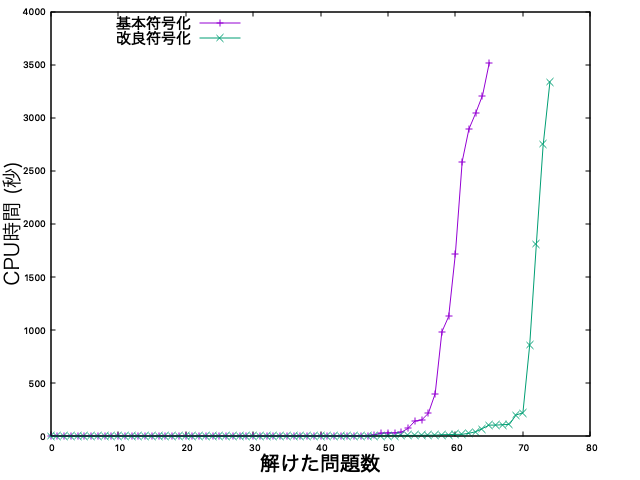
\includegraphics[scale=0.38]{fig/cactus.png}
 \end{figure}\vfill

\begin{itemize}
 \item 改良符号化は,基本符号化と比較して,より多くの問題を高速に解いている.
\end{itemize}
\end{frame}

%%%%%%%%%%%%%%%%%%%%%%%%%%%%%%%%%%%%%%%%%%%%%%%%%%
%% 辺の数の表
%%%%%%%%%%%%%%%%%%%%%%%%%%%%%%%%%%%%%%%%%%%%%%%%%%
\begin{frame}{実験結果(2/2) : 解けた問題数による比較}

\begin{table}[t]
 \centering
 \begin{tabular}{r|c|c|c}
 \hline
 n& h(n)& 圧縮された解の個数& 圧縮率 \\
 \hline
 3&	1&	2&	1.3889 \\
 4&	3&	8&	0.3367 \\
 5&	4&	16&	0.0368 \\
 6&	7&	128&	0.0049 \\
 7&	9&	512&	0.0002 \\
 8&	13&	8192&	- \\
 9&	18&	262144&	- \\
 10&	23&	8388608&	- \\
 11&	29&	536870912&	- \\
 12&	36&	68719476736&	- \\
\end{tabular}
\caption{多色頂点数最大化問題の解の圧縮率}
\label{table:com}
\end{table}\vfill

\begin{itemize}
\item 辺の数が4,000を超える問題では,改良符号化がより多くの問題を解いている.
\item 改良符号化は,辺の数が40,000を超える問題も解けている.
\item 大規模な問題に対する改良符号化の優位性が確認できた.
\end{itemize}
\end{frame}
%%%%%%%%%%%%%%%%%%%%%%%%%%%%%%%%%%%%%%%%%%%%%%%%%%
%% 解の遷移問題
%%%%%%%%%%%%%%%%%%%%%%%%%%%%%%%%%%%%%%%%%%%%%%%%%%
\begin{frame}{遷移問題への拡張}

\begin{alertblock}{根付き全域森遷移問題}
  根付き全域森問題とその2つの実行可能解が与えられたとき,
  ある解から他のもう一つの解へ根付き全域森の制約を満たしながら移る
  ``解の遷移問題''.
  \begin{itemize}
  \item 各ステップ$t$で変更可能な辺の数を$d$個以下に制限し(\textbf{遷移制約})
  \item 最短ステップ長での辺の変更手順を求めることが目的となる.
  \end{itemize}
\end{alertblock}
\vfill  
\begin{itemize}
\item ある配電網構成(スタート状態)から,他の配電網構成(ゴール状態)への
  スイッチの切替手順を求める問題に対応する.
\item 配電網における障害時の復旧予測への応用が期待できる.
\end{itemize} 
\end{frame}
%%%%%%%%%%%%%%%%%%%%%%%%%%%%%%%%%%%%%%%%%%%%%%%%%%
%% 遷移問題
%%%%%%%%%%%%%%%%%%%%%%%%%%%%%%%%%%%%%%%%%%%%%%%%%%
\begin{frame}{根付き全域森遷移問題の例}
  \begin{itemize}
  \item \structure{\bf 遷移制約}: 各ステップ$t$で変更可能な辺の数を
    $d=2$個以下とする.
  \end{itemize}
\begin{exampleblock}{}
 \begin{figure}[h]
  %\renewcommand{\arraystretch}{0.9}
  \tabcolsep = 3mm  
  \centering
  \begin{tabular}{ccc}
   \onslide<1-> $t=0$ (スタート状態) & & \onslide<2> $t=1$\\
   \onslide<1-> \scalebox{0.8}{%%%%%%%%%%%%%%%%%%%%%%%%%%%%%%%%%%%%%%%%%%%%%%%%%%
% 実行例(t=0) (第6章で使う)
%%%%%%%%%%%%%%%%%%%%%%%%%%%%%%%%%%%%%%%%%%%%%%%%%%

\begin{tikzpicture}[x=1.5cm,y=1.5cm,scale=0.7]

 % 設定
 \tikzset{root/.style={circle,draw=black,fill=gray!30,minimum size=1cm}}
 \tikzset{node/.style={circle,draw=black,minimum size=1cm}}
 
 % 補助線
 % \draw [help lines,blue,step=2cm] (-3,0) grid (3,-3);

 % 時間 %
 % \node[rectangle,draw=black] at (-3,1) {$t=0$};

 % root %
 \node[root] at (-2,0) (1){$c_1$};
 \node[above=0.5cm] at (1) {$r_1$};
 \node[root] at (2,0) (3){$c_3$};
 \node[above=0.5cm] at (3) {$r_3$};

 % node %
 \node[node] at (0,0) (2){$c_2$};
 \node[node] at (-2,-2) (4){$c_4$};
 \node[node] at (0,-2) (5){$c_5$};
 \node[node] at (2,-2) (6){$c_6$};

 % 繋がっていない辺は破線
 %\foreach \u / \v in {2/3, 2/5, 4/5}
 %\draw [dashed] (\u) -- (\v);
 % 繋がってる辺は実線
 \foreach \u / \v in {1/2, 1/4, 3/6, 5/6}
 \draw (\u) -- (\v);

 % スイッチ switch %
  \node at (-1,0.2) {$s_1$};
 % \node at (1,0.2) {$s_2$};
  \node at (-2.2,-1) {$s_3$};
 % \node at (-0.2,-1) {$s_4$};
  \node at (1.8,-1) {$s_5$};
 % \node at (-1,-1.8) {$s_6$};
  \node at (1,-1.8) {$s_7$};
 %

\end{tikzpicture}

%%%%%%%%%%%%%%%%%%%%%%%%%%%%%%%%%%%%%%%%%%%%%%%%%%%%%%%%%%
%%% Local Variables:
%%% mode: japanese-latex
%%% TeX-master: paper.tex
%%% End:
}
   & \onslide<2> \lw{$\Rightarrow$} & 
	\onslide<2> \scalebox{0.8}{%%%%%%%%%%%%%%%%%%%%%%%%%%%%%%%%%%%%%%%%%%%%%%%%%%
% 実行例(t=1) (第6章で使う)
%%%%%%%%%%%%%%%%%%%%%%%%%%%%%%%%%%%%%%%%%%%%%%%%%%

\begin{tikzpicture}[x=1.5cm,y=1.5cm,scale=0.7]

 % 設定
 \tikzset{root/.style={circle,draw=black,fill=gray!30,minimum size=1cm}}
 \tikzset{node/.style={circle,draw=black,minimum size=1cm}}
 
 % 補助線
 % \draw [help lines,blue,step=2cm] (-3,0) grid (3,-3);

 % 時間 %
 % \node[rectangle,draw=black] at (-3,1) {$t=1$};

 % root %
 \node[root] at (-2,0) (1){$c_1$};
 \node[above=0.5cm] at (1) {$r_1$};
 \node[root] at (2,0) (3){$c_3$};
 \node[above=0.5cm] at (3) {$r_3$};

 % node %
 \node[node] at (0,0) (2){$c_2$};
 \node[node] at (-2,-2) (4){$c_4$};
 \node[node] at (0,-2) (5){$c_5$};
 \node[node] at (2,-2) (6){$c_6$};

 % 繋がっていない辺は破線
 %\foreach \u / \v in {2/3, 2/5, 4/5}
 %\draw [dashed] (\u) -- (\v);
 % 繋がってる辺は実線
 \foreach \u / \v in {2/3, 1/4, 3/6, 5/6}
 \draw (\u) -- (\v);

 % スイッチ switch %
 % \node at (-1,0.2) {$s_1$};
 %
 \node at (1,0.2) {$s_2$};
 \node at (-2.2,-1) {$s_3$};
 % \node at (-0.2,-1) {$s_4$};
 \node at (1.8,-1) {$s_5$};
 % \node at (-1,-1.8) {$s_6$};
 \node at (1,-1.8) {$s_7$};
 %

\end{tikzpicture}

%%%%%%%%%%%%%%%%%%%%%%%%%%%%%%%%%%%%%%%%%%%%%%%%%%%%%%%%%%
%%% Local Variables:
%%% mode: japanese-latex
%%% TeX-master: paper.tex
%%% End:
}\\
   & & \onslide<2> \lower1ex\hbox{$\Downarrow$} \\
   & & \\
   \onslide<1-> \scalebox{0.8}{%%%%%%%%%%%%%%%%%%%%%%%%%%%%%%%%%%%%%%%%%%%%%%%%%%
% 実行例(t=3) (第6章で使う)
%%%%%%%%%%%%%%%%%%%%%%%%%%%%%%%%%%%%%%%%%%%%%%%%%%
\begin{tikzpicture}[scale=0.6]

 % 設定
 \tikzset{node/.style={circle,draw=black,fill=white}}

 \definecolor{edge1}{RGB}{191,0,0}
 \definecolor{node1}{RGB}{249,200,200}
 \definecolor{edge3}{RGB}{38,38,134}
 \definecolor{node3}{RGB}{200,200,249}

 % 補助線
 % \draw [help lines,blue] (0,0) grid (20,6);

 % node %
 \node[circle, ultra thick, draw=edge1, fill=node1](out1){1};
 \node[node, fill=node3, right=of out1] (out2){2};
 \node[circle, ultra thick, draw=edge3,fill=node3, right=of out2](out3){3};
 \node[node, fill=node3, below=of out1] (out4){4};
 \node[node, fill=node3, below=of out2] (out5){5};
 \node[node, fill=node3, below=of out3] (out6){6};

 \foreach \u / \v in {}
 \draw [very thick, edge1] (\u) -- (\v);

 \foreach \u / \v in {out2/out3,out2/out5,out4/out5,out5/out6}
 \draw [very thick, edge3](\u) -- (\v);
\end{tikzpicture}

%%%%%%%%%%%%%%%%%%%%%%%%%%%%%%%%%%%%%%%%%%%%%%%%%%%%%%%%%%
%%% Local Variables:
%%% mode: japanese-latex
%%% TeX-master: paper.tex
%%% End:
}
   & \onslide<2> \lw{$\Leftarrow$} &
   \onslide<2> \scalebox{0.8}{%%%%%%%%%%%%%%%%%%%%%%%%%%%%%%%%%%%%%%%%%%%%%%%%%%
% 実行例(t=2) (第6章で使う)
%%%%%%%%%%%%%%%%%%%%%%%%%%%%%%%%%%%%%%%%%%%%%%%%%%

\begin{tikzpicture}[x=1.5cm,y=1.5cm,scale=0.7]

 % 設定
 \tikzset{root/.style={circle,draw=black,fill=gray!30,minimum size=1cm}}
 \tikzset{node/.style={circle,draw=black,minimum size=1cm}}
 
 % 補助線
 % \draw [help lines,blue,step=2cm] (-3,0) grid (3,-3);

 % 時間 %
 % \node[rectangle,draw=black] at (-3,1) {$t=2$};

 % root %
 \node[root] at (-2,0) (1){$1$};
% \node[above=0.5cm] at (1) {$r_1$};
 \node[root] at (2,0) (3){$3$};
 %\node[above=0.5cm] at (3) {$r_3$};

 % node %
 \node[node] at (0,0) (2){$2$};
 \node[node] at (-2,-2) (4){$4$};
 \node[node] at (0,-2) (5){$5$};
 \node[node] at (2,-2) (6){$6$};

 % 繋がっていない辺は破線
 %\foreach \u / \v in {2/3, 2/5, 4/5}
 %\draw [dashed] (\u) -- (\v);
 % 繋がってる辺は実線
 \foreach \u / \v in {2/3, 4/5, 3/6, 5/6}
 \draw (\u) -- (\v);

 % スイッチ switch %
 % \node at (-1,0.2) {$s_1$};
 % \node at (1,0.2) {$s_2$};
 % \node at (-2.2,-1) {$s_3$};
 % \node at (-0.2,-1) {$s_4$};
 % \node at (1.8,-1) {$s_5$};
 % \node at (-1,-1.8) {$s_6$};
 % \node at (1,-1.8) {$s_7$};
 %

\end{tikzpicture}

%%%%%%%%%%%%%%%%%%%%%%%%%%%%%%%%%%%%%%%%%%%%%%%%%%%%%%%%%%
%%% Local Variables:
%%% mode: japanese-latex
%%% TeX-master: paper.tex
%%% End:
}\\
   \onslide<1->$t= \only<1>{\ ?} \only<2>{\structure{\bf 3}} $ (ゴール状態) 
   & & \onslide<2> $t=2$
  \end{tabular}
 \end{figure}
\end{exampleblock}
\end{frame}
%%%%%%%%%%%%%%%%%%%%%%%%%%%%%%%%%%%%%%%%%%%%%%%%%%
%% 提案アプローチ
%%%%%%%%%%%%%%%%%%%%%%%%%%%%%%%%%%%%%%%%%%%%%%%%%%
\begin{frame}{提案手法}
  \begin{itemize}
  \item 根付き全域森遷移問題のASP符号化を2種類考案した.
  \end{itemize}
  \begin{block}{シングルショット符号化 (改良符号化の自然な拡張)}
    \begin{itemize}
    \item 与えられたステップ長$t$の解が存在するかを判定する.
      % \begin{itemize}
      % \item 与えられたステップ長$t$の解が存在するかを判定する.
      % \item 各アトムにステップ長を表す項\code{T}を追加.例) \code{inForest(X,Y,T)}
      % \item スタート状態,ゴール状態,遷移制約に関するルールを追加.
      % \end{itemize}
    \item 解が見つかるまで,ステップ長$t$を増やしながら,複数の問題を
      繰り返し解く必要がある.
    \item 各問題中の制約の大部分は共通であるため,
      \textbf{同一の探索空間を何度も調べる}ことになり,
      \textbf{求解効率が低下}するという問題点がある.
  \end{itemize}
 \end{block}
 \vfill
 \begin{alertblock}{マルチショット符号化}
   \begin{itemize}
   \item ASPシステム\textit{clingo}のマルチショット解法ライブラリを使用.
   \item 同様の探索失敗を避けるために獲得した学習節を保持することによって,
		 \textbf{無駄な探索を行うことなく},制約を追加した論理プログラムを
		 連続的に解くことができる.
  \end{itemize}
 \end{alertblock}

\end{frame}
%%%%%%%%%%%%%%%%%%%%%%%%%%%%%%%%%%%%%%%%%%%%%%%%%%
%% 実験内容--遷移問題
%%%%%%%%%%%%%%%%%%%%%%%%%%%%%%%%%%%%%%%%%%%%%%%%%%
\begin{frame}{実験概要}
  \renewcommand{\thefootnote}{\fnsymbol{footnote}}
  \setcounter{footnote}{1}
  提案手法の有効性を評価するために,以下の実験を行った.
  \vfill
  \begin{itemize}
  \item \structure{\bf 比較するASP符号化:}
    \begin{itemize}
    \item シングルショット符号化
    \item マルチショット符号化
    \end{itemize}
  \item \structure{\bf ベンチマーク問題:} 全30問
    \begin{itemize}
    \item DNET\footnote{https://github.com/takemaru/dnet}
      で公開されている実用規模の配電網問題(\textsf{fukui-tepco},
      スイッチ数 468,変電所の数 72)をベース
    \item 実行可能解の中から,スタート状態を5つ,ゴール状態を6つをラン
      ダムに選択して使用
    \end{itemize}
  \item \structure{\bf ASPシステム:} \textit{clingo-5.4.0} $+$ \textit{trendy}
  \item \structure{\bf 実験環境:} Mac mini,3.2GHz Intel Core i7,64GBメモリ
  \end{itemize}
\end{frame}
%%%%%%%%%%%%%%%%%%%%%%%%%%%%%%%%%%%%%%%%%%%%%%%%%%
%% 実験結果--遷移問題
%%%%%%%%%%%%%%%%%%%%%%%%%%%%%%%%%%%%%%%%%%%%%%%%%%
\begin{frame}{実験結果:CPU時間の比較(1/2)}
 \centering
 \scalebox{0.8}{\begin{tabular}{ccrrr}  
 \rowcolor[RGB]{0,96,0}
  \color{white}問題名 &
  \multicolumn{1}{c}{\color{white}ステップ長$t$} & 
  \multicolumn{1}{c}{\color{white}シングルショット} & 
  \multicolumn{1}{c}{\color{white}マルチショット} & 
  \multicolumn{1}{c}{\color{white}シングル/マルチ} \\
 \rowcolor[RGB]{230,239,230}%%
s1\_g60 & 8 & 50.098 & \alert{25.659} & 1.952~ \\
 \rowcolor[RGB]{196,230,196}%
s1\_g70 & 8 & 47.177 & \alert{24.981} & 1.889~ \\
 \rowcolor[RGB]{230,239,230}%%
s1\_g80 & 8 & 43.193 & \alert{15.852} & 2.725~ \\
 \rowcolor[RGB]{196,230,196}%
s1\_g90 & 8 & 48.984 & \alert{22.983} & 2.131~ \\
 \rowcolor[RGB]{230,239,230}%%
s1\_g100 & 6 & 20.964 & \alert{4.709} & 4.452~ \\
 \rowcolor[RGB]{196,230,196}%
s10\_g60 & 6 & 21.947 & \alert{5.132} & 4.277~ \\
 \rowcolor[RGB]{230,239,230}%%
s10\_g70 & 8 & 43.840 & \alert{16.290} & 2.691~ \\
 \rowcolor[RGB]{196,230,196}%
s10\_g80 & 6 & 21.156 & \alert{4.887} & 4.329~ \\
 \rowcolor[RGB]{230,239,230}%%
s10\_g90 & 6 & 21.276 & \alert{5.324} & 3.996~ \\
 \rowcolor[RGB]{196,230,196}%
s10\_g100 & 8 & 45.704 & \alert{17.697} & 2.583~ \\
 \rowcolor[RGB]{230,239,230}%%
s20\_g60 & 6 & 21.202 & \alert{4.973} & 4.263~ \\
 \rowcolor[RGB]{196,230,196}%
s20\_g70 & 4 & 9.890 & \alert{2.699} & 3.664~ \\
 \rowcolor[RGB]{230,239,230}%%
s20\_g80 & 8 & 48.473 & \alert{16.335} & 2.967~ \\
 \rowcolor[RGB]{196,230,196}%
s20\_g90 & 10 & 107.938 & \alert{64.441} & 1.675~ \\
 \rowcolor[RGB]{230,239,230}%%
s20\_g100 & 8 & 48.473 & \alert{17.894} & 2.709~ \\
 \rowcolor[RGB]{196,230,196}%
s30\_g60 & 6 & 21.189 & \alert{5.287} & 4.008~ \\
 \rowcolor[RGB]{230,239,230}%%
s30\_g70 & 4 & 9.901 & \alert{2.735} & 3.620~ \\
 \rowcolor[RGB]{196,230,196}%
s30\_g80 & 6 & 21.884 & \alert{5.223} & 4.196~ \\
 \rowcolor[RGB]{230,239,230}%%
s30\_g90 & 4 & 9.979 & \alert{2.658} & 3.754~ \\
 \rowcolor[RGB]{196,230,196}%
s30\_g100 & 8 & 50.344 & \alert{18.845} & 2.671~ \\
\end{tabular}
}
\end{frame}

\begin{frame}{実験結果:CPU時間の比較(2/2)}
 \centering
 \vskip -2ex
 \scalebox{0.8}{\begin{tabular}{ccrrr}  
 \rowcolor[RGB]{0,96,0}
  \color{white}問題名 &
  \multicolumn{1}{c}{\color{white}ステップ長$t$} & 
  \multicolumn{1}{c}{\color{white}シングルショット} & 
  \multicolumn{1}{c}{\color{white}マルチショット} & 
  \multicolumn{1}{c}{\color{white}シングル/マルチ} \\
 \rowcolor[RGB]{230,239,230}
 s40\_g60 & 8 & 44.637 & \alert{14.254} & 3.132~ \\
 \rowcolor[RGB]{196,230,196}%
s40\_g70 & 6 & 21.334 & \alert{4.795} & 4.449~ \\
 \rowcolor[RGB]{230,239,230}
s40\_g80 & 8 & 45.202 & \alert{14.099} & 3.206~ \\
 \rowcolor[RGB]{196,230,196}%
s40\_g90 & 6 & 21.710 & \alert{5.119} & 4.241~ \\
 \rowcolor[RGB]{230,239,230}
s40\_g100 & 6 & 21.299 & \alert{5.666} & 3.759~ \\
  \rowcolor[RGB]{196,230,196}%
s50\_g60 & 4 & 10.021 & \alert{2.726} & 3.676~ \\
\rowcolor[RGB]{230,239,230}
s50\_g70 & 6 & 21.291 & \alert{4.718} & 4.513~ \\
 \rowcolor[RGB]{196,230,196}%
s50\_g80 & 6 & 21.163 & \alert{6.503} & 3.254~ \\
 \rowcolor[RGB]{230,239,230}
s50\_g90 & 10 & 108.299 & \alert{65.352} & 1.657~ \\
 \rowcolor[RGB]{196,230,196}%
s50\_g100 & 4 & 9.934 & \alert{2.700} & 3.679~ \\
 \noalign{\hrule height 0.5pt} \rowcolor[RGB]{230,239,230}
\multicolumn{2}{c}{平均} & 34.617 & \alert{13.685} & 3.337~ \\
\end{tabular}}
 
 \vskip 1em
\begin{itemize}
 \item マルチショット符号化は,シングルショット符号化と比較して,全ての
	   問題をより高速に解いており,\alert{\bf 平均で3.3倍の高速化}を実現している.
 \item 最短ステップ長$t=10$の問題も解けることが確認できた.
\end{itemize}
\end{frame}
%%%%%%%%%%%%%%%%%%%%%%%%%%%%%%%%%%%%%%%%%%%%%%%%%%
%% まとめ
%%%%%%%%%%%%%%%%%%%%%%%%%%%%%%%%%%%%%%%%%%%%%%%%%%
\begin{frame}{まとめ}
\begin{alertblock}{}
  根付き全域森問題(トポロジ制約のみの配電網問題に対応)に対して,解集合
  プログラミング(ASP)を用いた手法を提案し,その有用性を確認した.
\end{alertblock}
\begin{itemize}
\item \structure{\bf 記述性: }
  ASPの高い表現力により,根付き全域森問題の制約を簡潔に表現できること
  を確認した(ASPのルールで6個).
\item \structure{\bf 効率性: }
  辺の数が40,000を超えるような問題も解くことができ,
  大規模な問題に対する改良符号化の優位性を確認できた.
\item \structure{\bf 拡張性: }
  遷移問題への拡張を行い,マルチショットASP解法の有効性を確認できた.
\end{itemize}
\vfill
\begin{block}{今後の課題}
  \begin{itemize}
  \item 電気制約への対応.
  \item 根付き全域森遷移問題の更なる性能改善
    \begin{itemize}
    \item ASPシステム\textit{clingo}の変数選択ヒューリスティクスの利用
    \end{itemize}
  \end{itemize}
 \end{block}
\end{frame}
%###########################################################
%##### 補助スライド ########################################
%###########################################################

%%%%%%%%%%%%%%%%%%%%%%%%%%%%%%%%%%%%%%%%%%%%%%%%%%
%% 第2部 開始
%%%%%%%%%%%%%%%%%%%%%%%%%%%%%%%%%%%%%%%%%%%%%%%%%%
\begin{frame}{~}
\centering \Large
\textbf{-- 根付き全域森遷移問題のデモ --}
\end{frame}
%%%%%%%%%%%%%%%%%%%%%%%%%%%%%%%%%%%%%%%%%%%%%%%%%%
%% 遷移問題の入力 (グラフ)
%%%%%%%%%%%%%%%%%%%%%%%%%%%%%%%%%%%%%%%%%%%%%%%%%%
\begin{frame}{問題:入力グラフ}
  \renewcommand{\thefootnote}{\fnsymbol{footnote}}
  \setcounter{footnote}{1}
\begin{textblock*}{\linewidth}(5pt,40pt)
\begin{itemize}
 \item DNET\footnote{https://github.com/takemaru/dnet}
	   \!の例(\code{data/test.yaml})を使用
\end{itemize} 
\end{textblock*}\vfill
\begin{textblock*}{0.4\linewidth}(223pt,25pt)
 \centering
 \fbox{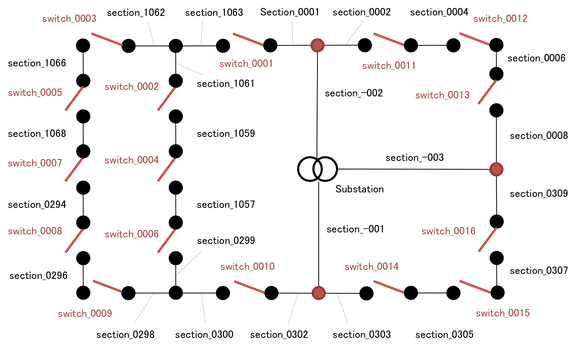
\includegraphics[width=\linewidth]{fig/dnet.png}}
 {\tiny(https://github.com/takemaru/dnetより引用)}
\end{textblock*}\vfill
\scalebox{0.75}{%%%%%%%%%%%%%%%%%%%%%%%%%%%%%%%%%%%%%%%%%%%%%%%%%%
% test.lp
%%%%%%%%%%%%%%%%%%%%%%%%%%%%%%%%%%%%%%%%%%%%%%%%%%

\begin{tikzpicture}

 % 設定
 \tikzset{node/.style={circle,draw=black,fill=white,minimum height=1cm}}

 \definecolor{edgeR}{RGB}{191,0,0}
 \definecolor{nodeR}{RGB}{249,200,200}
 \definecolor{edgeY}{RGB}{255,149,0}
 \definecolor{nodeY}{RGB}{255,231,76}
 \definecolor{edgeB}{RGB}{38,38,134}
 \definecolor{nodeB}{RGB}{200,200,249}

 \tikzset{NodeR/.style={circle,draw=black,fill=nodeR,minimum height=1cm}}
 \tikzset{NodeY/.style={circle,draw=black,fill=nodeY,minimum height=1cm}}
 \tikzset{NodeB/.style={circle,draw=black,fill=nodeB,minimum height=1cm}}

 % 補助線
 % \draw [help lines,blue] (0,0) grid (20,6);

 % 入力されるグラフ
 % node %
 \node[node, ultra thick,draw=edgeR,fill=nodeR] (1) {1};
 \node[node,left= of 1] (2){2};
 \node[node,above= of 2] (3){3};
 \node[node,left= of 2] (4){4};
 \node[node,above= of 3] (5){5};
 \node[node,left= of 3] (6){6};
 \node[node,above= of 5] (7){7};
 \node[node,left= of 5] (8){8};
 \node[node,left= of 7] (9){9};
 \node[node,right= of 7, ultra thick,draw=edgeB,fill=nodeB] (10){10};
 \node[node,right= of 1] (11){11};
 \node[node,right= of 11] (12){12};
 \node[node,above=2cm of 12, ultra thick,draw=edgeY,fill=nodeY] (13){13};
 \node[node,right= of 10] (14){14};
 \node[node,right= of 14] (15){15};

 %\node[rectangle,above=2cm of 1, draw=black,ultra thick,minimum height=1cm] (ss){変電所};

 % 辺
 \foreach \u / \v in {1/2,2/3,2/4,3/5,4/6,5/7,6/8,8/9,7/9,7/10,1/11,11/12,12/13,13/15,14/15,10/14}
 \draw (\u) -- (\v);
\end{tikzpicture}

%%%%%%%%%%%%%%%%%%%%%%%%%%%%%%%%%%%%%%%%%%%%%%%%%%%%%%%%%%
%%% Local Variables:
%%% mode: japanese-latex
%%% TeX-master: ``slide''
%%% End:
}
\begin{textblock*}{0.4\linewidth}(225pt,150pt)
\begin{itemize}
 \item \structure{\bf ノード数: 15}
 \item \structure{\bf 辺数: 16}
 \item \structure{\bf 根ノード数: 3}
\end{itemize}
\end{textblock*}\vfill
\end{frame}
%%%%%%%%%%%%%%%%%%%%%%%%%%%%%%%%%%%%%%%%%%%%%%%%%%
%% 遷移問題の入力 (スタートとゴール)
%%%%%%%%%%%%%%%%%%%%%%%%%%%%%%%%%%%%%%%%%%%%%%%%%%
\begin{frame}{問題:スタート状態とゴール状態}
  \begin{columns}
    \begin{column}{0.45\textwidth}\centering
      \begin{exampleblock}{スタート状態}
	\centering
	\scalebox{0.55}{%%%%%%%%%%%%%%%%%%%%%%%%%%%%%%%%%%%%%%%%%%%%%%%%%%
% test.lp
%%%%%%%%%%%%%%%%%%%%%%%%%%%%%%%%%%%%%%%%%%%%%%%%%%

\begin{tikzpicture}

 % 設定
 \tikzset{node/.style={circle,draw=black,fill=white,minimum height=1cm}}

 \definecolor{edgeR}{RGB}{191,0,0}
 \definecolor{nodeR}{RGB}{249,200,200}
 \definecolor{edgeY}{RGB}{255,149,0}
 \definecolor{nodeY}{RGB}{255,231,76}
 \definecolor{edgeB}{RGB}{38,38,134}
 \definecolor{nodeB}{RGB}{200,200,249}

 \tikzset{NodeR/.style={circle,draw=black,fill=nodeR,minimum height=1cm}}
 \tikzset{NodeY/.style={circle,draw=black,fill=nodeY,minimum height=1cm}}
 \tikzset{NodeB/.style={circle,draw=black,fill=nodeB,minimum height=1cm}}

 % 補助線
 % \draw [help lines,blue] (0,0) grid (20,6);

 % 入力されるグラフ
 % node %
 \node[node, ultra thick,draw=edgeR,fill=nodeR] (1) {1};
 \node[node,left= of 1] (2){2};
 \node[node,above= of 2] (3){3};
 \node[node,left= of 2] (4){4};
 \node[node,above= of 3] (5){5};
 \node[node,left= of 3] (6){6};
 \node[node,above= of 5] (7){7};
 \node[node,left= of 5] (8){8};
 \node[node,left= of 7] (9){9};
 \node[node,right= of 7, ultra thick,draw=edgeB,fill=nodeB] (10){10};
 \node[node,right= of 1] (11){11};
 \node[node,right= of 11] (12){12};
 \node[node,above=2cm of 12, ultra thick,draw=edgeY,fill=nodeY] (13){13};
 \node[node,right= of 10] (14){14};
 \node[node,right= of 14] (15){15};

 %\node[rectangle,above=2cm of 1, draw=black,ultra thick,minimum height=1cm] (ss){変電所};

 % 辺
 % root1
 \foreach \u / \v in {}
 \draw [very thick, edgeR] (\u) -- (\v);
 \foreach \n in {}
 \node[NodeR] at (\n) {\n};
 % root10
 \foreach \u / \v in {10/7,7/9,9/8,8/6,7/5,4/6,2/4,3/2}
 \draw [very thick, edgeB](\u) -- (\v);
 \foreach \n in {7,9,8,6,5,4,3,2}
 \node[NodeB] at (\n) {\n};
 % root13
 \foreach \u / \v in {13/15, 14/15,13/12,11/12}
 \draw [very thick, edgeY] (\u) -- (\v);
 \foreach \n in {15,14,12,11}
 \node[NodeY] at (\n) {\n};

\end{tikzpicture}

%%%%%%%%%%%%%%%%%%%%%%%%%%%%%%%%%%%%%%%%%%%%%%%%%%%%%%%%%%
%%% Local Variables:
%%% mode: japanese-latex
%%% TeX-master: ``slide''
%%% End:
}
      \end{exampleblock}
    \end{column}
    \begin{column}{0.05\textwidth}\centering
      $\Rightarrow$
    \end{column}
    \begin{column}{0.45\textwidth}\centering
      \begin{exampleblock}{ゴール状態}
        \centering
        \scalebox{0.55}{%%%%%%%%%%%%%%%%%%%%%%%%%%%%%%%%%%%%%%%%%%%%%%%%%%
% test.lp
%%%%%%%%%%%%%%%%%%%%%%%%%%%%%%%%%%%%%%%%%%%%%%%%%%

\begin{tikzpicture}

 % 設定
 \tikzset{node/.style={circle,draw=black,fill=white,minimum height=1cm}}

 \definecolor{edgeR}{RGB}{191,0,0}
 \definecolor{nodeR}{RGB}{249,200,200}
 \definecolor{edgeY}{RGB}{255,149,0}
 \definecolor{nodeY}{RGB}{255,231,76}
 \definecolor{edgeB}{RGB}{38,38,134}
 \definecolor{nodeB}{RGB}{200,200,249}

 \tikzset{NodeR/.style={circle,draw=black,fill=nodeR,minimum height=1cm}}
 \tikzset{NodeY/.style={circle,draw=black,fill=nodeY,minimum height=1cm}}
 \tikzset{NodeB/.style={circle,draw=black,fill=nodeB,minimum height=1cm}}

 % 補助線
 % \draw [help lines,blue] (0,0) grid (20,6);

 % 入力されるグラフ
 % node %
 \node[node, ultra thick,draw=edgeR,fill=nodeR] (1) {1};
 \node[node,left= of 1] (2){2};
 \node[node,above= of 2] (3){3};
 \node[node,left= of 2] (4){4};
 \node[node,above= of 3] (5){5};
 \node[node,left= of 3] (6){6};
 \node[node,above= of 5] (7){7};
 \node[node,left= of 5] (8){8};
 \node[node,left= of 7] (9){9};
 \node[node,right= of 7, ultra thick,draw=edgeB,fill=nodeB] (10){10};
 \node[node,right= of 1] (11){11};
 \node[node,right= of 11] (12){12};
 \node[node,above=2cm of 12, ultra thick,draw=edgeY,fill=nodeY] (13){13};
 \node[node,right= of 10] (14){14};
 \node[node,right= of 14] (15){15};

 %\node[rectangle,above=2cm of 1, draw=black,ultra thick,minimum height=1cm] (ss){変電所};

 % 辺
 % root1
 \foreach \u / \v in {1/2,4/6,2/4,3/2,3/5,1/11}
 \draw [very thick, edgeR] (\u) -- (\v);
 \foreach \n in {2,3,4,5,6,11}
 \node[NodeR] at (\n) {\n};
 %root10
 \foreach \u / \v in {10/7,7/9,9/8,10/14,14/15}
 \draw [very thick, edgeB](\u) -- (\v);
 \foreach \n in {7,9,8,14,15}
 \node[NodeB] at (\n) {\n};
 % root13
 \foreach \u / \v in {13/12}
 \draw [very thick, edgeY] (\u) -- (\v);
 \foreach \n in {12}
 \node[NodeY] at (\n) {\n};


\end{tikzpicture}

%%%%%%%%%%%%%%%%%%%%%%%%%%%%%%%%%%%%%%%%%%%%%%%%%%%%%%%%%%
%%% Local Variables:
%%% mode: japanese-latex
%%% TeX-master: ``slide''
%%% End:
}
      \end{exampleblock}
    \end{column}
  \end{columns}\vfill
\begin{itemize}
 \item 問題のASPファクト形式,遷移問題の符号化は\textit{emacs}にて 
\end{itemize}
\end{frame}
%%%%%%%%%%%%%%%%%%%%%%%%%%%%%%%%%%%%%%%%%%%%%%%%%%
%% 遷移問題の実行
%%%%%%%%%%%%%%%%%%%%%%%%%%%%%%%%%%%%%%%%%%%%%%%%%%
\begin{frame}{遷移}
\begin{itemize}
 \only<1>{\item $t=0$ \structure{\bf スタート状態}}
 \only<2>{\item $t=1$}
 \only<3>{\item $t=2$}
 \only<4>{\item $t=3$}
 \only<5>{\item $t=4$ \structure{\bf ゴール状態}}
\end{itemize}\vfill
 \begin{exampleblock}{}
\centering
%%%%%%%%%%%%%%%%%%%%%%%%%%%%%%%%%%%%%%%%%%%%%%%%%%
% test.lp
%%%%%%%%%%%%%%%%%%%%%%%%%%%%%%%%%%%%%%%%%%%%%%%%%%

\begin{tikzpicture}

 % 設定
 \tikzset{node/.style={circle,draw=black,fill=white,minimum height=1cm}}

 \definecolor{edgeR}{RGB}{191,0,0}
 \definecolor{nodeR}{RGB}{249,200,200}
 \definecolor{edgeY}{RGB}{255,149,0}
 \definecolor{nodeY}{RGB}{255,231,76}
 \definecolor{edgeB}{RGB}{38,38,134}
 \definecolor{nodeB}{RGB}{200,200,249}

 \tikzset{NodeR/.style={circle,draw=black,fill=nodeR,minimum height=1cm}}
 \tikzset{NodeY/.style={circle,draw=black,fill=nodeY,minimum height=1cm}}
 \tikzset{NodeB/.style={circle,draw=black,fill=nodeB,minimum height=1cm}}

 % 補助線
 % \draw [help lines,blue] (0,0) grid (20,6);

 % 入力されるグラフ
 % node %
 \node[node, ultra thick,draw=edgeR,fill=nodeR] (1) {1};
 \node[node,left= of 1] (2){2};
 \node[node,above= of 2] (3){3};
 \node[node,left= of 2] (4){4};
 \node[node,above= of 3] (5){5};
 \node[node,left= of 3] (6){6};
 \node[node,above= of 5] (7){7};
 \node[node,left= of 5] (8){8};
 \node[node,left= of 7] (9){9};
 \node[node,right= of 7, ultra thick,draw=edgeB,fill=nodeB] (10){10};
 \node[node,right= of 1] (11){11};
 \node[node,right= of 11] (12){12};
 \node[node,above=2cm of 12, ultra thick,draw=edgeY,fill=nodeY] (13){13};
 \node[node,right= of 10] (14){14};
 \node[node,right= of 14] (15){15};

 %\node[rectangle,above=2cm of 1, draw=black,ultra thick,minimum height=1cm] (ss){変電所};

 \onslide<1>
 % 辺
 % root1
 \foreach \u / \v in {}
 \draw [very thick, edgeR] (\u) -- (\v);
 \foreach \n in {}
 \node[NodeR] at (\n) {\n};
 % root10
 \foreach \u / \v in {10/7,7/9,9/8,8/6,7/5,4/6,2/4,3/2}
 \draw [very thick, edgeB](\u) -- (\v);
 \foreach \n in {7,9,8,6,5,4,3,2}
 \node[NodeB] at (\n) {\n};
 % root13
 \foreach \u / \v in {13/15, 14/15,13/12,11/12}
 \draw [very thick, edgeY] (\u) -- (\v);
 \foreach \n in {15,14,12,11}
 \node[NodeY] at (\n) {\n};

 \onslide<2>
 % 辺
 % root1
 \foreach \u / \v in {1/2,4/6,2/4,3/2}
 \draw [very thick, edgeR] (\u) -- (\v);
 \foreach \n in {2,3,4,6}
 \node[NodeR] at (\n) {\n};
 % root10
 \foreach \u / \v in {10/7,7/9,9/8,7/5}
 \draw [very thick, edgeB](\u) -- (\v);
 \foreach \n in {7,9,8,5}
 \node[NodeB] at (\n) {\n};
 % root13
 \foreach \u / \v in {13/15, 14/15,13/12,11/12}
 \draw [very thick, edgeY] (\u) -- (\v);
 \foreach \n in {15,14,12,11}
 \node[NodeY] at (\n) {\n};

 \onslide<3>
 % 辺
 % root1
 \foreach \u / \v in {1/2,4/6,2/4,3/2}
 \draw [very thick, edgeR] (\u) -- (\v);
 \foreach \n in {2,3,4,6}
 \node[NodeR] at (\n) {\n};
 % root10
 \foreach \u / \v in {10/7,7/9,9/8,7/5,10/14,14/15}
 \draw [very thick, edgeB](\u) -- (\v);
 \foreach \n in {7,9,8,5,14,15}
 \node[NodeB] at (\n) {\n};
 % root13
 \foreach \u / \v in {13/12,11/12}
 \draw [very thick, edgeY] (\u) -- (\v);
 \foreach \n in {12,11}
 \node[NodeY] at (\n) {\n};

 \onslide<4>
 % 辺
 % root1
 \foreach \u / \v in {1/2,4/6,2/4,3/2,3/5}
 \draw [very thick, edgeR] (\u) -- (\v);
 \foreach \n in {2,3,4,5,6}
 \node[NodeR] at (\n) {\n};
 %root10
 \foreach \u / \v in {10/7,7/9,9/8,10/14,14/15}
 \draw [very thick, edgeB](\u) -- (\v);
 \foreach \n in {7,9,8,14,15}
 \node[NodeB] at (\n) {\n};
 % root13
 \foreach \u / \v in {13/12,11/12}
 \draw [very thick, edgeY] (\u) -- (\v);
 \foreach \n in {12,11}
 \node[NodeY] at (\n) {\n};

 \onslide<5>
 % 辺
 % root1
 \foreach \u / \v in {1/2,4/6,2/4,3/2,3/5,1/11}
 \draw [very thick, edgeR] (\u) -- (\v);
 \foreach \n in {2,3,4,5,6,11}
 \node[NodeR] at (\n) {\n};
 %root10
 \foreach \u / \v in {10/7,7/9,9/8,10/14,14/15}
 \draw [very thick, edgeB](\u) -- (\v);
 \foreach \n in {7,9,8,14,15}
 \node[NodeB] at (\n) {\n};
 % root13
 \foreach \u / \v in {13/12}
 \draw [very thick, edgeY] (\u) -- (\v);
 \foreach \n in {12}
 \node[NodeY] at (\n) {\n};

 \onslide<1->

\end{tikzpicture}

%%%%%%%%%%%%%%%%%%%%%%%%%%%%%%%%%%%%%%%%%%%%%%%%%%%%%%%%%%
%%% Local Variables:
%%% mode: japanese-latex
%%% TeX-master: ``slide''
%%% End:

\end{exampleblock}
\end{frame}





%###########################################################
%##### 補助スライド ########################################
%###########################################################

%%%% 補助スライド

\begin{frame}{~}
 \centering
 - 補足用 -
\end{frame} 

\begin{frame}{補足 : スマートグリッド}
 \begin{itemize}
  \item \structure{スマートグリッド}とは,電力の供給側,需要側において双方向の
		やり取りを可能にする次世代の\structure{賢い}電力網である.
  \item 従来と違い,通信技術の発達により,使用状況などを
		リアルタイムに把握することが可能となった.
  \item その時に応じた最適な配電網を構成し,制御するといったことが考えられている.
		\begin{itemize}
		 \item 電力需要の変化による,配電ロスの少ない構成.
		 \item 自然エネルギーによる発電量の変動を補う構成.
		\end{itemize}
  \item ASP言語の表現力や拡張性が,こうした条件の追加に活用できる可能性がある.
 \end{itemize}
\end{frame}

%%%%%%%%%%%%%%%%%%%%%%%%%%%%%%%%%%%%%%%%%%%%%%%%%%
%% 電気制約
%%%%%%%%%%%%%%%%%%%%%%%%%%%%%%%%%%%%%%%%%%%%%%%%%%
\begin{frame}{補足 : 電気制約}
 \begin{itemize}
  \item \alert{電気制約}は,送電する電流$\cdot$電圧の適正範囲を保証する制約.
  \begin{itemize}
   \item 供給経路の各区間で許容電流を超えない.
   \item 電気抵抗による電圧降下が許容範囲を超えない.
   \item etc.
  \end{itemize}
  \item 電流と電圧が影響し合う\structure{実数ドメイン上の制約}によって表される.
		% \begin{itemize}
		%  		 \item 送電システム上の条件など.
		% \end{itemize}
  \item 実数ドメイン上の制約は,純粋なASPのみで扱うのは\alert{困難}.
		\begin{itemize}
		 \item 緩和問題として,変電所から供給できる家庭の数に上限をつける.
		 \item ASPMT技術により,ASPで得られた解について,
			   背景理論ソルバーと連携して実数ドメイン上の制約を調べる.
		\end{itemize}
 \end{itemize}
\end{frame}


%%%%%%%%%%%%%%%%%%%%%%%%%%%%%%%%%%%%%%%%%%%%%%%%%%
%% 基礎化
%%%%%%%%%%%%%%%%%%%%%%%%%%%%%%%%%%%%%%%%%%%%%%%%%%
\begin{frame}{補足 : ASPシステム}
 
 \vspace{-0.5cm}

 \begin{figure}[htbp]
  \centering
  %%%%%%%%%%%%%%%%%%%%%%%%%%%%%%%%%%%%%%%%%%%%%%%%%%
%% 基礎化の流れの図
%%%%%%%%%%%%%%%%%%%%%%%%%%%%%%%%%%%%%%%%%%%%%%%%%%
\begin{tikzpicture}

 \definecolor{edge}{RGB}{38,38,134}
 \definecolor{node}{RGB}{220,220,249}

 \definecolor{alert_edge}{RGB}{191,0,0}
 \definecolor{alert_node}{RGB}{249,200,200}

 \definecolor{ex_edge}{RGB}{0,96,0}
 \definecolor{ex_node}{RGB}{230,239,230}

 \def\nodespace{2.4cm}

 \tikzset{block/.style={rectangle, thick, draw=edge, fill=node, text width=3cm, 
 text centered, rounded corners, text width=2cm, minimum height=1.5cm}};

 \tikzset{alertblock/.style={rectangle, thick, draw=alert_edge, fill=alert_node, 
 text width=3cm, text centered, rounded corners, text width=1.5cm, minimum height=1.2cm}};

 \node[block](ikkai){一階ASP\\プログラム};

 \node[rectangle,rounded corners, thick, draw=ex_edge, fill=ex_node, 
 right=0.22*\nodespace of ikkai, minimum width=6cm, minimum height=3cm, 
 text centered, label=ASPシステム](sys){};

 \node[block, right=\nodespace of ikkai](meidai){命題ASP\\プログラム};
 \node[block, right=\nodespace of meidai](ASP){解集合};

 \node[right=0.6*\nodespace of ikkai, text width=1.5cm, 
 text centered, text=red, anchor=south](){基礎化\\ソルバー};
 \node[right=0.4*\nodespace of meidai, text width=1.5cm, 
 text centered, text=red, anchor=south](){解集合\\ソルバー};

 
 \foreach \u / \v / \n in {ikkai/meidai,meidai/ASP}
 \draw [thick,->] (\u) to (\v);

\end{tikzpicture}
 \end{figure}

 \vspace{-0.5cm}

 \begin{exampleblock}{}
  \begin{enumerate}
   \item 一階ASPプログラムを基礎化ソルバーによって,
		 命題ASPプログラムに\alert{基礎化}する.
   \item 命題ASPプログラムについて,SAT技術を応用した解集合ソルバーが解集合を探索する.
  \end{enumerate}
 \end{exampleblock}

\end{frame}


%%%%%%%%%%%%%%%%%%%%%%%%%%%%%%%%%%%%%%%%%%%%%%%%%%
%% ASPのコード
%%%%%%%%%%%%%%%%%%%%%%%%%%%%%%%%%%%%%%%%%%%%%%%%%%
\begin{frame}[fragile]{補足 : 基本符号化のASPプログラム}
 \begin{exampleblock}{}
  \begin{center}
   %%%%%%%%%%%%%%%%%%%%%%%%%%%%%%%%%
   \lstinputlisting[numbers=left,%
   basicstyle=\ttfamily\tiny]{code/srf1.lp}
   %%%%%%%%%%%%%%%%%%%%%%%%%%%%%%%%% 
  \end{center}
 \end{exampleblock}
\end{frame}

\begin{frame}[fragile]{補足 : 改良符号化のASPプログラム}

 \begin{exampleblock}{}
  \begin{center}
   %%%%%%%%%%%%%%%%%%%%%%%%%%%%%%%%%
   \lstinputlisting[numbers=left,%
   basicstyle=\ttfamily\tiny]{code/srf2.lp}
   %%%%%%%%%%%%%%%%%%%%%%%%%%%%%%%%% 
  \end{center}
 \end{exampleblock}

\end{frame}



\end{document}
%%% Local Variables:
%%% mode: japanese-latex
%%% TeX-master: t
%%% End:
